\documentclass[journal]{style/vgtc}           % final (journal style)
%\documentclass[review,journal]{style/vgtc}         % review (journal style)
%\documentclass[widereview]{style/vgtc}             % wide-spaced review
%\documentclass[preprint,journal]{style/vgtc}       % preprint (journal style)
%\documentclass[electronic,journal]{style/vgtc}     % electronic version, journal

%% Uncomment one of the lines above depending on where your paper is
%% in the conference process. ``review'' and ``widereview'' are for review
%% submission, ``preprint'' is for pre-publication, and the final version
%% doesn't use a specific qualifier. Further, ``electronic'' includes
%% hyperreferences for more convenient online viewing.

%% Please use one of the ``review'' options in combination with the
%% assigned online id (see below) ONLY if your paper uses a double blind
%% review process. Some conferences, like IEEE Vis and InfoVis, have NOT
%% in the past.

%% Please note that the use of figures other than the optional teaser is not permitted on the first page
%% of the journal version.  Figures should begin on the second page and be
%% in CMYK or Grey scale format, otherwise, colour shifting may occur
%% during the printing process.  Papers submitted with figures other than the optional teaser on the
%% first page will be refused.

%% These three lines bring in essential packages: ``mathptmx'' for Type 1
%% typefaces, ``graphicx'' for inclusion of EPS figures. and ``times''
%% for proper handling of the times font family.

\usepackage{mathptmx}
\usepackage{graphicx}
\usepackage{times}

%% We encourage the use of mathptmx for consistent usage of times font
%% throughout the proceedings. However, if you encounter conflicts
%% with other math-related packages, you may want to disable it.

%% This turns references into clickable hyperlinks.
\usepackage[bookmarks,backref=true,linkcolor=black]{hyperref} %,colorlinks
\hypersetup{
  pdfauthor = {},
  pdftitle = {},
  pdfsubject = {},
  pdfkeywords = {},
  colorlinks=true,
  linkcolor= black,
  citecolor= black,
  pageanchor=true,
  urlcolor = black,
  plainpages = false,
  linktocpage
}

%% If you are submitting a paper to a conference for review with a double
%% blind reviewing process, please replace the value ``0'' below with your
%% OnlineID. Otherwise, you may safely leave it at ``0''.
\onlineid{0}

%% declare the category of your paper, only shown in review mode
\vgtccategory{Research}

%% allow for this line if you want the electronic option to work properly
\vgtcinsertpkg

%% In preprint mode you may define your own headline.
%\preprinttext{To appear in an IEEE VGTC sponsored conference.}

%% Paper title.

\title{Interactive Visual Analysis of Image-Centric Cohort Study Data}

%% This is how authors are specified in the journal style

%% indicate IEEE Member or Student Member in form indicated below
\author{TBA}
\authorfooter{
%% insert punctuation at end of each item
\item
 Otto-v.-Guericke-University Magdeburg
}

%other entries to be set up for journal
\shortauthortitle{Klemm \MakeLowercase{\textit{et al.}}: Interactive Visual Analytics of Image-Centric Cohort Study Data}
%\shortauthortitle{Firstauthor \MakeLowercase{\textit{et al.}}: Paper Title}

%% Abstract section.
\abstract{Epidemiological population studies impose information about a set of subjects (a \emph{cohort}) to characterize disease specific risk factors.
%
Cohort studies comprise heterogenous data variables describing the medical condition as well as demographic and lifestyle factors of a subject.
%
Using well established statistical methods the data is hypothesis driven analyzed to find statistically significant variable correlations ('\emph{interactions}').
%
Modern cohort studies also incorporate medical image data.
%
Analyzing these data requires image segmentation, extraction of key figures and shape based subject grouping.
\\
We propose a Interactive Visual Analytics approach that enables epidemiologists to examine both image-based as well as sociodemographic and medical attribute data.
%We propose a Interactive Visual Analytics approach to provide epidemiologists with the tools necessary to analyze this data.
%
It allows for both classical hypothesis validation approaches as well as hypothesis generation by incorporating data mining methods.
%
Adaptive linked information visualization views and 3d-shape renderings are combined with epidemiological techniques.
%
Similarity measures between data variables are used to compute interesting changes in variable interactions for the current variable selection.
%
Shape based grouping of subjects is facilitated using hierarchical agglomerative clustering. (Remove Clustering reference?)
} % end of abstract


%% Keywords that describe your work. Will show as 'Index Terms' in journal
%% please capitalize first letter and insert punctuation after last keyword
\keywords{Interactive Visual Analytics, Epidemiology}

%% ACM Computing Classification System (CCS). 
%% See <http://www.acm.org/class/1998/> for details.
%% The ``\CCScat'' command takes four arguments.

\CCScatlist{ % not used in journal version
 \CCScat{K.6.1}{Management of Computing and Information Systems}%
{Project and People Management}{Life Cycle};
 \CCScat{K.7.m}{The Computing Profession}{Miscellaneous}{Ethics}
}

%% Uncomment below to include a teaser figure.
  % \teaser{
  % \centering
  % \includegraphics[width=16cm]{CypressView}
  % \caption{In the Clouds: Vancouver from Cypress Mountain.}
  % }

%% Uncomment below to disable the manuscript note
%\renewcommand{\manuscriptnotetxt}{}

%% Copyright space is enabled by default as required by guidelines.
%% It is disabled by the 'review' option or via the following command:
% \nocopyrightspace

%%%%%%%%%%%%%%%%%%%%%%%%%%%%%%%%%%%%%%%%%%%%%%%%%%%%%%%%%%%%%%%%
%%%%%%%%%%%%%%%%%%%%%% START OF THE PAPER %%%%%%%%%%%%%%%%%%%%%%
%%%%%%%%%%%%%%%%%%%%%%%%%%%%%%%%%%%%%%%%%%%%%%%%%%%%%%%%%%%%%%%%%

\begin{document}

%% The ``\maketitle'' command must be the first command after the
%% ``begin{document}'' command. It prepares and prints the title block.

%% the only exception to this rule is the \firstsection command
\firstsection{Introduction}

\maketitle

%% \section{Introduction} %for journal use above \firstsection{..} instead
Epidemiology aims to characterize health and disease by determining risk factors.
%
Clinical problems and questions answered using epidemiological methods comprise diagnosis accuracy, disease frequency, risk factors, disease prognosis, effectiveness of treatments or preventions and cause of diseases \cite{Fletcher2012}.
%
%Cohort studies are a epidemiological method to gather data about a group of subjects (a \emph{cohort)}) to make general statements about these problems.
%
Observations made by clinicians in the daily routine are translated into hypothesis.
%
These are used to determine environmental and lifestyle factors are as well as medical attributes which are believed to influence a condition of interest.
%
The data variables necessary are gathered using interviews and clinical examinations.
%
Statistical methods like regression analysis aim aim to check the attribute list for plausibility.
%

Longitudinal population-based studies like the Study of Health in Pomerania \cite{Volzke2011} aim to gather as much information as possible about a defined sample of people (a \emph{cohort}).
%
The sample is drawn randomized to avoid selection bias prohibit statements based on statistical correlations in the cohort to be inferred to the whole population.
%
Also a information bias needs to be avoided by strictly standardizing the data acquisition.
%
Statistical correlations are also prone to confounding, meaning that two factors influence each other and therefore should be normalized with respect to each other.
%
When for example one investigates risk factors for prostate cancer in male subjects the outcome is strongly dependent on the age.
%
Therefore results need to be age adjusted to be comparable.
%
Confounding variables, however, are often not obvious at all and characterizing them is already an epidemiological result.
\\\\
Modern cohort studies often include medical image data which introduces new problems.
%
Since it is unethical to expose people to radiation, non-harming imaging like Magnetic Resonance Imaging (MRI) or Ultrasound Imaging is used.
%
As MRI scans are expensive there exists a tradeoff between quality of the image data and their associated costs.
%
To quantify these data it is necessary to segment it.
%
Manual segmentation via radiological experts is possible but very costly and prone to inter- and intra observer variability.
%
Segmentation algorithms allow for (semi)-automated analysis of the data but require sophisticated methods due to high inter-subject variability caused by the subject diversity.
%
Analyzing spatial data with other epidemiological factors require techniques which reach beyond standard statistical methods.
\\
We propose a Interactive Visual Analysis approach to provide a way to analyze both image- and non-image data.
%
Visual queries and direct feedback of Visual Analytics systems allow for a fast exploration of the data space.
%
Intended as a extension to the well established epidemiological tools it provides a way to rapidly validate hypothesis as well as trigger hypothesis generation using Data Mining methods such as clustering.
%


%Interactive Visual Analysis (IVA) TODO QUELLE provides techniques which not only show promising potential for combining both 3d visualization with 

Our contributions are:
\begin{itemize}
	\item Applying the Interactive Visual Analysis approach to the epidemiological problem domain by characterizing special affordances of this context.
	\item Provide an overview over the workflow for analyzing cohort study data to gain insigth into the large subject spaces.
	\item Provide Visualization Techniques which combine both Information Visualization and 3D Rendering of Organ Shapes as well as combining them with well known epidemiological graphics and key figures.
	\item Implement the presented methods in a Web Framework based on WebGL, D3js and Nodejs as backend.
\end{itemize}

%Statistical correlations derived from analyzing the data itself may be misleading since 

%Include Implementation details - web based; how are image data included; what technologies are used?

\section{Medical and Technical Background}
In this section we want to give insight into the epidemiological workflow when analyzing cohort study data to identify the problems we address in this paper.
%
ToDo Define Epidemiological Outcome
%
\subsection{Epidemiological Workflow}
Epidemiologists follow a strict workflow mainly driven by statistic tools to validate hypothesis.
%
Following Thew and colleagues publication on this matter, the workflow can be characterized as follows.
%
Hypothesis most commonly base on observations made by clinicians in their daily routine.
%
A set of attributes depicting conditions affected by the hypothesis is compiled accordingly.
%
Confounding variables need to be adjusted so that they do not affect the effect size of a attribute.
%
Statistical methods such as regression analysis are applied to measure the effect size of attributes to the outcome of interest.
%

Reproducibility of results is an epidemiological key requirement.
%
Longitudinal epidemiological studies require the acquired attributes to be comparable to evaluate them.
%
If the data acquisition process changes, a information bias is introduced to the data, disallowing inference between acquisition cycles.
%
This underlines the high quality standards to methods processing the data, whether to extract additional parameters or gain insight.
%
To determine, whether a subject is prone to be affected by a certain disease, relative risks a expressed through the evaluation of p values which indicate statistical significance.
%
Statistics tools such as SPSS and STATA play a major role for analyzing epidemiolgical data. 
%
Graphic data representation is largely used to show results rather than gaining insight.

Bernhards Paper\\
- Missing Data\\
- Follow-Up Questions?\\
- grouping essentiell\\
- problems when analyzing image data\\
	- what are Problems there\\
	- how can shape be included?\\
	- show image data of multiple subjects
	
\subsection{Epidemiological Data}
Benrhard Paper
- sociodemographic data
- medical data
- pain indicators
- DATA TYPES
	- dichotomous data

	
\paragraph{Image acquisition}: standardization of MR Scanners

\subsection{The Study of Health in Pomerania (SHIP)}


\section{Prior and Related Work}
- VMV Paper\\
- Analysis of data in the Rotterdam study\\
- VA in Epidemiology Part of Bernhards Paper\\
	- Commercial visual Analytics Systems\\
- GPloms\\
Unterlagen Wissenschaftliche Projekt

\section{Interactive Visual Analytics in Cohort Study Data}
\begin{figure}[htb]
 \centering
 %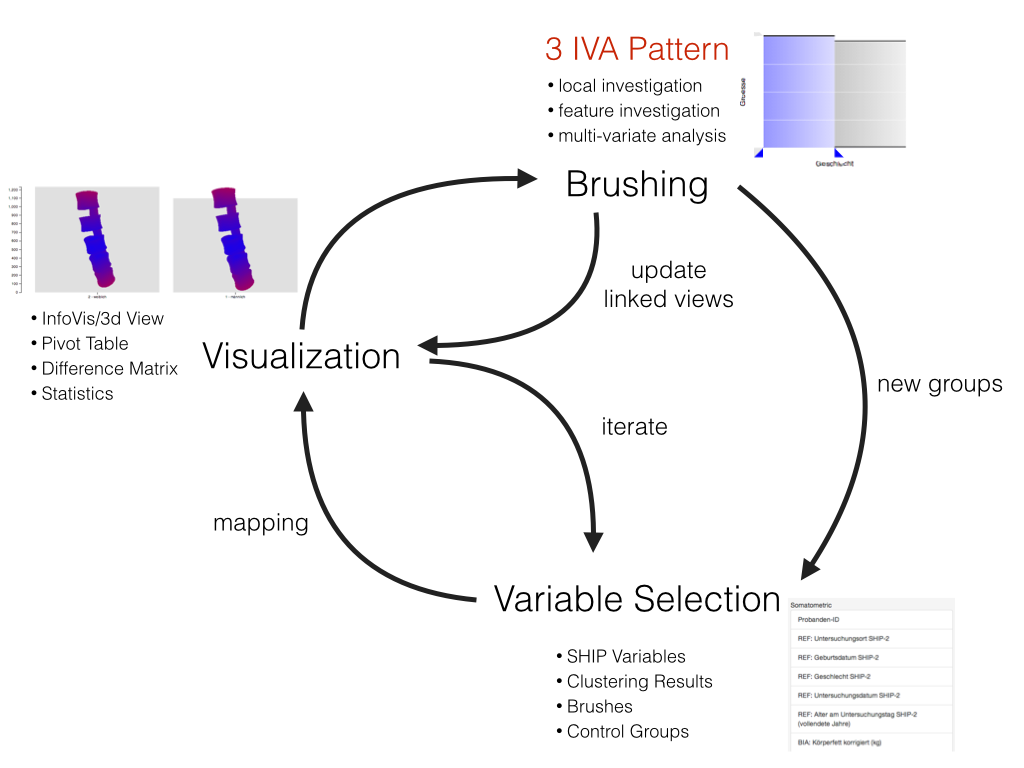
\includegraphics[width=1.5in]{figures/InteractionLoop}
 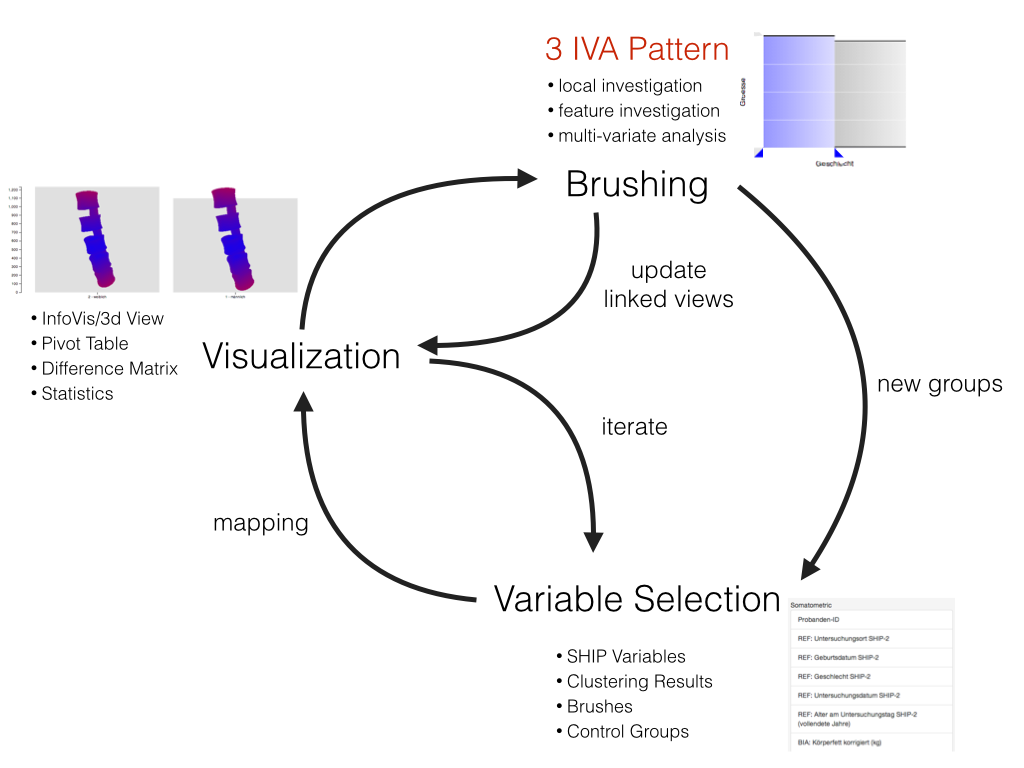
\includegraphics[width=3.0in]{figures/InteractionLoop}
 \caption{Interaction Overview}
\end{figure}

According to Steffens Terminology in Interactive Visual Analysis of Perfusion Data
\\\\
\textbf{Object Space}\\
- Medical Image Data / Spine Segmentations\\
\textbf{Attribute Space}\\
- SHIP-Variables\\
- Derived visualizations

? Where to incorporate Levels of IVA

\subsection{Feature Localization}
- Projection from Image Space to Attribute data. This is more difficult in our application, because we currently only brush on derived features.\\
- Clustering in Image Space yields Groups which can be analyzed using the attribute space\\
- Create a Pipeline Overview over different Levels of different IVA Patterns and Stages

\subsection{Local Investigation}
- Selection of Information using Bar Charts, Scatterplots or Parallel Coordinates which projects the selection into the Object space\\
- this selection is for categorical data already given implicitly bei projecting the 3D-View onto the Bar Charts/Mosaik Plots!\\
- this aims to locale features of the data!\\
- Gain Information about SHIP-Variables by putting them into the context of each other. The Pivot Table allows for direct numerical\\ analysis, while the information visualizations allow for better insight of the combination

\subsection{Multivariate Analysis}
- Selection of Elements in Scatterplots, Barcharts or Parallel Coordinates Views - observe how selection changes another view - this allows for multivariate analysis\\
- Becker, R.A., Cleveland, W.S.: Brushing scatterplots. Technometrics 29(2) (1987)\\
- Wang Baldonado, M.Q., Woodruff, A., Kuchinsky, A.: Guidelines for using multiple views in information visualization. In: AVI ’00: Proceedings of the working conference on Ad- vanced visual interfaces, pp. 110–119. ACM Press, New York, NY, USA (2000). DOI\\ http://doi.acm.org/10.1145/345513.345271
- By brushing individual parameters or create new binnings of parameter it is possible to see how they change in coordinated views. This is already implemented in the Cargo framework\\
- by creating comparative 3d Visualizations it is possible to assess the influence of non-image parameters to the visual space.

\subsection{Implementation}
Diagram of used Technologies

\section{Application}

\subsection{The Spine Dataset}
- Describe steps from gathering Information from the raw image files (segmentation, abstraction, visualization)\\
- Input of Epidemiologists goes here!

\section{Summary and Conclusion}


%% if specified like this the section will be committed in review mode
\acknowledgments{SHIP is part of the Community Medicine Research net of the University of Greifswald, Germany, which is funded by the Federal Ministry of Education and Research (grant no. 03ZIK012), the Ministry of Cultural Affairs as well as the Social Ministry of the Federal State of Mecklenburg-West Pomerania. Whole-body MR imaging was supported by a joint grant from Siemens Healthcare, Erlangen, Germany and the Federal State of Mecklenburg-Vorpommern. The University of Greifswald is a member of the ‘Centre of Knowledge Interchange’ program of the Siemens AG. This work was supported by the DFG Priority Program 1335: Scalable Visual Analytics.}

\bibliographystyle{abbrv}
%%use following if all content of bibtex file should be shown
%\nocite{*}
\bibliography{bibliography}
\end{document}
